\documentclass[1p]{elsarticle_modified}
%\bibliographystyle{elsarticle-num}

%\usepackage[colorlinks]{hyperref}
%\usepackage{abbrmath_seonhwa} %\Abb, \Ascr, \Acal ,\Abf, \Afrak
\usepackage{amsfonts}
\usepackage{amssymb}
\usepackage{amsmath}
\usepackage{amsthm}
\usepackage{scalefnt}
\usepackage{amsbsy}
\usepackage{kotex}
\usepackage{caption}
\usepackage{subfig}
\usepackage{color}
\usepackage{graphicx}
\usepackage{xcolor} %% white, black, red, green, blue, cyan, magenta, yellow
\usepackage{float}
\usepackage{setspace}
\usepackage{hyperref}

\usepackage{tikz}
\usetikzlibrary{arrows}

\usepackage{multirow}
\usepackage{array} % fixed length table
\usepackage{hhline}

%%%%%%%%%%%%%%%%%%%%%
\makeatletter
\renewcommand*\env@matrix[1][\arraystretch]{%
	\edef\arraystretch{#1}%
	\hskip -\arraycolsep
	\let\@ifnextchar\new@ifnextchar
	\array{*\c@MaxMatrixCols c}}
\makeatother %https://tex.stackexchange.com/questions/14071/how-can-i-increase-the-line-spacing-in-a-matrix
%%%%%%%%%%%%%%%

\usepackage[normalem]{ulem}

\newcommand{\msout}[1]{\ifmmode\text{\sout{\ensuremath{#1}}}\else\sout{#1}\fi}
%SOURCE: \msout is \stkout macro in https://tex.stackexchange.com/questions/20609/strikeout-in-math-mode

\newcommand{\cancel}[1]{
	\ifmmode
	{\color{red}\msout{#1}}
	\else
	{\color{red}\sout{#1}}
	\fi
}

\newcommand{\add}[1]{
	{\color{blue}\uwave{#1}}
}

\newcommand{\replace}[2]{
	\ifmmode
	{\color{red}\msout{#1}}{\color{blue}\uwave{#2}}
	\else
	{\color{red}\sout{#1}}{\color{blue}\uwave{#2}}
	\fi
}

\newcommand{\Sol}{\mathcal{S}} %segment
\newcommand{\D}{D} %diagram
\newcommand{\A}{\mathcal{A}} %arc


%%%%%%%%%%%%%%%%%%%%%%%%%%%%%5 test

\def\sl{\operatorname{\textup{SL}}(2,\Cbb)}
\def\psl{\operatorname{\textup{PSL}}(2,\Cbb)}
\def\quan{\mkern 1mu \triangleright \mkern 1mu}

\theoremstyle{definition}
\newtheorem{thm}{Theorem}[section]
\newtheorem{prop}[thm]{Proposition}
\newtheorem{lem}[thm]{Lemma}
\newtheorem{ques}[thm]{Question}
\newtheorem{cor}[thm]{Corollary}
\newtheorem{defn}[thm]{Definition}
\newtheorem{exam}[thm]{Example}
\newtheorem{rmk}[thm]{Remark}
\newtheorem{alg}[thm]{Algorithm}

\newcommand{\I}{\sqrt{-1}}
\begin{document}

%\begin{frontmatter}
%
%\title{Boundary parabolic representations of knots up to 8 crossings}
%
%%% Group authors per affiliation:
%\author{Yunhi Cho} 
%\address{Department of Mathematics, University of Seoul, Seoul, Korea}
%\ead{yhcho@uos.ac.kr}
%
%
%\author{Seonhwa Kim} %\fnref{s_kim}}
%\address{Center for Geometry and Physics, Institute for Basic Science, Pohang, 37673, Korea}
%\ead{ryeona17@ibs.re.kr}
%
%\author{Hyuk Kim}
%\address{Department of Mathematical Sciences, Seoul National University, Seoul 08826, Korea}
%\ead{hyukkim@snu.ac.kr}
%
%\author{Seokbeom Yoon}
%\address{Department of Mathematical Sciences, Seoul National University, Seoul, 08826,  Korea}
%\ead{sbyoon15@snu.ac.kr}
%
%\begin{abstract}
%We find all boundary parabolic representation of knots up to 8 crossings.
%
%\end{abstract}
%\begin{keyword}
%    \MSC[2010] 57M25 
%\end{keyword}
%
%\end{frontmatter}

%\linenumbers
%\tableofcontents
%
\newcommand\colored[1]{\textcolor{white}{\rule[-0.35ex]{0.8em}{1.4ex}}\kern-0.8em\color{red} #1}%
%\newcommand\colored[1]{\textcolor{white}{ #1}\kern-2.17ex	\textcolor{white}{ #1}\kern-1.81ex	\textcolor{white}{ #1}\kern-2.15ex\color{red}#1	}

{\Large $\underline{12n_{0612}~(K12n_{0612})}$}

\setlength{\tabcolsep}{10pt}
\renewcommand{\arraystretch}{1.6}
\vspace{1cm}\begin{tabular}{m{100pt}>{\centering\arraybackslash}m{274pt}}
\multirow{5}{120pt}{
	\centering
	\includegraphics[width=112pt]{../../../GIT/diagram.site/Diagrams/png/2701_12n_0612.png}\\
\ \ \ A knot diagram\footnotemark}&
\allowdisplaybreaks
\textbf{Linearized knot diagam} \\
\cline{2-2}
 &
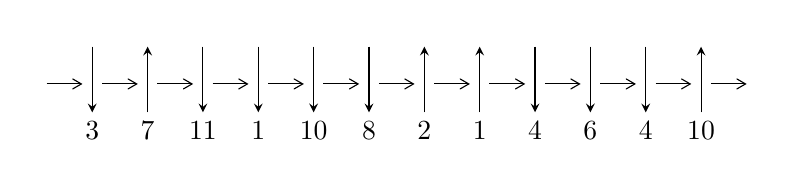
\begin{tikzpicture}[x=20pt, y=17pt]
	% nodes
	\node (C0) at (0, 0) {};
	\node (C1) at (1, 0) {};
	\node (C1U) at (1, +1) {};
	\node (C1D) at (1, -1) {3};

	\node (C2) at (2, 0) {};
	\node (C2U) at (2, +1) {};
	\node (C2D) at (2, -1) {7};

	\node (C3) at (3, 0) {};
	\node (C3U) at (3, +1) {};
	\node (C3D) at (3, -1) {11};

	\node (C4) at (4, 0) {};
	\node (C4U) at (4, +1) {};
	\node (C4D) at (4, -1) {1};

	\node (C5) at (5, 0) {};
	\node (C5U) at (5, +1) {};
	\node (C5D) at (5, -1) {10};

	\node (C6) at (6, 0) {};
	\node (C6U) at (6, +1) {};
	\node (C6D) at (6, -1) {8};

	\node (C7) at (7, 0) {};
	\node (C7U) at (7, +1) {};
	\node (C7D) at (7, -1) {2};

	\node (C8) at (8, 0) {};
	\node (C8U) at (8, +1) {};
	\node (C8D) at (8, -1) {1};

	\node (C9) at (9, 0) {};
	\node (C9U) at (9, +1) {};
	\node (C9D) at (9, -1) {4};

	\node (C10) at (10, 0) {};
	\node (C10U) at (10, +1) {};
	\node (C10D) at (10, -1) {6};

	\node (C11) at (11, 0) {};
	\node (C11U) at (11, +1) {};
	\node (C11D) at (11, -1) {4};

	\node (C12) at (12, 0) {};
	\node (C12U) at (12, +1) {};
	\node (C12D) at (12, -1) {10};
	\node (C13) at (13, 0) {};

	% arrows
	\draw[->,>={angle 60}]
	(C0) edge (C1) (C1) edge (C2) (C2) edge (C3) (C3) edge (C4) (C4) edge (C5) (C5) edge (C6) (C6) edge (C7) (C7) edge (C8) (C8) edge (C9) (C9) edge (C10) (C10) edge (C11) (C11) edge (C12) (C12) edge (C13) ;	\draw[->,>=stealth]
	(C1U) edge (C1D) (C2D) edge (C2U) (C3U) edge (C3D) (C4U) edge (C4D) (C5U) edge (C5D) (C6U) edge (C6D) (C7D) edge (C7U) (C8D) edge (C8U) (C9U) edge (C9D) (C10U) edge (C10D) (C11U) edge (C11D) (C12D) edge (C12U) ;
	\end{tikzpicture} \\
\hhline{~~} \\& 
\textbf{Solving Sequence} \\ \cline{2-2} 
 &
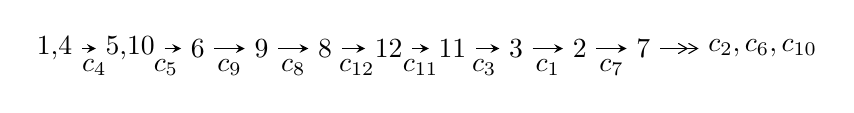
\begin{tikzpicture}[x=23pt, y=7pt]
	% node
	\node (A0) at (-1/8, 0) {1,4};
	\node (A1) at (17/16, 0) {5,10};
	\node (A2) at (17/8, 0) {6};
	\node (A3) at (25/8, 0) {9};
	\node (A4) at (33/8, 0) {8};
	\node (A5) at (41/8, 0) {12};
	\node (A6) at (49/8, 0) {11};
	\node (A7) at (57/8, 0) {3};
	\node (A8) at (65/8, 0) {2};
	\node (A9) at (73/8, 0) {7};
	\node (C1) at (1/2, -1) {$c_{4}$};
	\node (C2) at (13/8, -1) {$c_{5}$};
	\node (C3) at (21/8, -1) {$c_{9}$};
	\node (C4) at (29/8, -1) {$c_{8}$};
	\node (C5) at (37/8, -1) {$c_{12}$};
	\node (C6) at (45/8, -1) {$c_{11}$};
	\node (C7) at (53/8, -1) {$c_{3}$};
	\node (C8) at (61/8, -1) {$c_{1}$};
	\node (C9) at (69/8, -1) {$c_{7}$};
	\node (A10) at (11, 0) {$c_{2},c_{6},c_{10}$};

	% edge
	\draw[->,>=stealth]	
	(A0) edge (A1) (A1) edge (A2) (A2) edge (A3) (A3) edge (A4) (A4) edge (A5) (A5) edge (A6) (A6) edge (A7) (A7) edge (A8) (A8) edge (A9) ;
	\draw[->>,>={angle 60}]	
	(A9) edge (A10);
\end{tikzpicture} \\ 

\end{tabular} \\

\footnotetext{
The image of knot diagram is generated by the software ``\textbf{Draw programme}" developed by Andrew Bartholomew(\url{http://www.layer8.co.uk/maths/draw/index.htm\#Running-draw}), where we modified some parts for our purpose(\url{https://github.com/CATsTAILs/LinksPainter}).
}\phantom \\ \newline 
\centering \textbf{Ideals for irreducible components\footnotemark of $X_{\text{par}}$} 
 
\begin{align*}
I^u_{1}&=\langle 
b- u,\\
\phantom{I^u_{1}}&\phantom{= \langle  }65065875226664520 u^{27}+9394396496362895 u^{26}+\cdots+76364734116743 a+26735659168418070,\\
\phantom{I^u_{1}}&\phantom{= \langle  }u^{28}+23 u^{26}+\cdots-3 u+1\rangle \\
I^u_{2}&=\langle 
b+u,\;5 u^{16}+u^{15}+\cdots+a-5,\\
\phantom{I^u_{2}}&\phantom{= \langle  }u^{17}+3 u^{15}- u^{14}-4 u^{13}-5 u^{11}+5 u^{10}+11 u^9-6 u^8-2 u^7-2 u^6-7 u^5+8 u^4+5 u^3-5 u^2- u+1\rangle \\
I^u_{3}&=\langle 
1.90741\times10^{76} u^{35}+2.50394\times10^{76} u^{34}+\cdots+5.34816\times10^{78} b-7.63438\times10^{78},\\
\phantom{I^u_{3}}&\phantom{= \langle  }4.20379\times10^{66} u^{35}+2.74371\times10^{66} u^{34}+\cdots+1.04184\times10^{69} a-1.38242\times10^{70},\\
\phantom{I^u_{3}}&\phantom{= \langle  }u^{36}+u^{35}+\cdots-2560 u+121\rangle \\
\\
\end{align*}
\raggedright * 3 irreducible components of $\dim_{\mathbb{C}}=0$, with total 81 representations.\\
\footnotetext{All coefficients of polynomials are rational numbers. But the coefficients are sometimes approximated in decimal forms when there is not enough margin.}
\newpage
\renewcommand{\arraystretch}{1}
\centering \section*{I. $I^u_{1}= \langle b- u,\;6.51\times10^{16} u^{27}+9.39\times10^{15} u^{26}+\cdots+7.64\times10^{13} a+2.67\times10^{16},\;u^{28}+23 u^{26}+\cdots-3 u+1 \rangle$}
\flushleft \textbf{(i) Arc colorings}\\
\begin{tabular}{m{7pt} m{180pt} m{7pt} m{180pt} }
\flushright $a_{1}=$&$\begin{pmatrix}0\\u\end{pmatrix}$ \\
\flushright $a_{4}=$&$\begin{pmatrix}1\\0\end{pmatrix}$ \\
\flushright $a_{5}=$&$\begin{pmatrix}1\\u^2\end{pmatrix}$ \\
\flushright $a_{10}=$&$\begin{pmatrix}-852.041 u^{27}-123.020 u^{26}+\cdots-1960.13 u-350.105\\u\end{pmatrix}$ \\
\flushright $a_{6}=$&$\begin{pmatrix}-104.065 u^{27}+370.478 u^{26}+\cdots-4216.19 u+1309.36\\-42.7858 u^{27}+67.8173 u^{26}+\cdots-845.364 u+240.781\end{pmatrix}$ \\
\flushright $a_{9}=$&$\begin{pmatrix}-852.041 u^{27}-123.020 u^{26}+\cdots-1959.13 u-350.105\\u\end{pmatrix}$ \\
\flushright $a_{8}=$&$\begin{pmatrix}-852.041 u^{27}-123.020 u^{26}+\cdots-1959.13 u-350.105\\240.781 u^{27}+42.7858 u^{26}+\cdots+483.981 u+123.020\end{pmatrix}$ \\
\flushright $a_{12}=$&$\begin{pmatrix}-456.322 u^{27}+18.9555 u^{26}+\cdots-1801.95 u+59.0018\\-240.781 u^{27}-42.7858 u^{26}+\cdots-481.981 u-123.020\end{pmatrix}$ \\
\flushright $a_{11}=$&$\begin{pmatrix}-697.103 u^{27}-23.8304 u^{26}+\cdots-2283.93 u-64.0183\\-240.781 u^{27}-42.7858 u^{26}+\cdots-481.981 u-123.020\end{pmatrix}$ \\
\flushright $a_{3}=$&$\begin{pmatrix}-186.897 u^{27}+111.670 u^{26}+\cdots-1633.52 u+381.526\\80.2342 u^{27}-172.964 u^{26}+\cdots+2060.86 u-611.260\end{pmatrix}$ \\
\flushright $a_{2}=$&$\begin{pmatrix}643.875 u^{27}+247.704 u^{26}+\cdots-217.453 u+810.960\\-403.888 u^{27}+1.74743 u^{26}+\cdots-1518.50 u+43.0095\end{pmatrix}$ \\
\flushright $a_{7}=$&$\begin{pmatrix}20.8672 u^{27}-274.777 u^{26}+\cdots+2601.82 u-917.955\\-35.7010 u^{27}+222.640 u^{26}+\cdots-2384.15 u+774.366\end{pmatrix}$\\&\end{tabular}
\flushleft \textbf{(ii) Obstruction class $= -1$}\\~\\
\flushleft \textbf{(iii) Cusp Shapes $= -\frac{57088194451595465}{76364734116743} u^{27}+\frac{88581311353921087}{76364734116743} u^{26}+\cdots-\frac{1111026347572146836}{76364734116743} u+\frac{313608959053702506}{76364734116743}$}\\~\\
\newpage\renewcommand{\arraystretch}{1}
\flushleft \textbf{(iv) u-Polynomials at the component}\newline \\
\begin{tabular}{m{50pt}|m{274pt}}
Crossings & \hspace{64pt}u-Polynomials at each crossing \\
\hline $$\begin{aligned}c_{1},c_{6}\end{aligned}$$&$\begin{aligned}
&u^{28}+9 u^{27}+\cdots+84 u+16
\end{aligned}$\\
\hline $$\begin{aligned}c_{2},c_{7}\end{aligned}$$&$\begin{aligned}
&u^{28}+5 u^{27}+\cdots+2 u+4
\end{aligned}$\\
\hline $$\begin{aligned}c_{3},c_{5},c_{10}\\c_{11}\end{aligned}$$&$\begin{aligned}
&u^{28}+u^{27}+\cdots+4 u+1
\end{aligned}$\\
\hline $$\begin{aligned}c_{4},c_{9}\end{aligned}$$&$\begin{aligned}
&u^{28}+23 u^{26}+\cdots+3 u+1
\end{aligned}$\\
\hline $$\begin{aligned}c_{8}\end{aligned}$$&$\begin{aligned}
&u^{28}-25 u^{27}+\cdots-98862 u+9028
\end{aligned}$\\
\hline $$\begin{aligned}c_{12}\end{aligned}$$&$\begin{aligned}
&u^{28}+21 u^{27}+\cdots+3584 u+512
\end{aligned}$\\
\hline
\end{tabular}\\~\\
\newpage\renewcommand{\arraystretch}{1}
\flushleft \textbf{(v) Riley Polynomials at the component}\newline \\
\begin{tabular}{m{50pt}|m{274pt}}
Crossings & \hspace{64pt}Riley Polynomials at each crossing \\
\hline $$\begin{aligned}c_{1},c_{6}\end{aligned}$$&$\begin{aligned}
&y^{28}+21 y^{27}+\cdots+2064 y+256
\end{aligned}$\\
\hline $$\begin{aligned}c_{2},c_{7}\end{aligned}$$&$\begin{aligned}
&y^{28}+9 y^{27}+\cdots+84 y+16
\end{aligned}$\\
\hline $$\begin{aligned}c_{3},c_{5},c_{10}\\c_{11}\end{aligned}$$&$\begin{aligned}
&y^{28}-11 y^{27}+\cdots-6 y+1
\end{aligned}$\\
\hline $$\begin{aligned}c_{4},c_{9}\end{aligned}$$&$\begin{aligned}
&y^{28}+46 y^{27}+\cdots+49 y+1
\end{aligned}$\\
\hline $$\begin{aligned}c_{8}\end{aligned}$$&$\begin{aligned}
&y^{28}-3 y^{27}+\cdots+785869044 y+81504784
\end{aligned}$\\
\hline $$\begin{aligned}c_{12}\end{aligned}$$&$\begin{aligned}
&y^{28}-17 y^{27}+\cdots+4456448 y+262144
\end{aligned}$\\
\hline
\end{tabular}\\~\\
\newpage\flushleft \textbf{(vi) Complex Volumes and Cusp Shapes}
$$\begin{array}{c|c|c}  
\text{Solutions to }I^u_{1}& \I (\text{vol} + \sqrt{-1}CS) & \text{Cusp shape}\\
 \hline 
\begin{aligned}
u &= -0.062917 + 0.794694 I \\
a &= -1.44001 - 0.70376 I \\
b &= -0.062917 + 0.794694 I\end{aligned}
 & -1.93668 - 4.60321 I & -5.64825 + 3.26019 I \\ \hline\begin{aligned}
u &= -0.062917 - 0.794694 I \\
a &= -1.44001 + 0.70376 I \\
b &= -0.062917 - 0.794694 I\end{aligned}
 & -1.93668 + 4.60321 I & -5.64825 - 3.26019 I \\ \hline\begin{aligned}
u &= \phantom{-}0.193820 + 0.693750 I \\
a &= \phantom{-}1.312680 - 0.250146 I \\
b &= \phantom{-}0.193820 + 0.693750 I\end{aligned}
 & -0.409488 - 0.484105 I & -3.68035 + 2.98454 I \\ \hline\begin{aligned}
u &= \phantom{-}0.193820 - 0.693750 I \\
a &= \phantom{-}1.312680 + 0.250146 I \\
b &= \phantom{-}0.193820 - 0.693750 I\end{aligned}
 & -0.409488 + 0.484105 I & -3.68035 - 2.98454 I \\ \hline\begin{aligned}
u &= -0.015958 + 0.620215 I \\
a &= -2.15814 - 0.25579 I \\
b &= -0.015958 + 0.620215 I\end{aligned}
 & -5.53121 + 1.96442 I & -8.05770 - 3.63784 I \\ \hline\begin{aligned}
u &= -0.015958 - 0.620215 I \\
a &= -2.15814 + 0.25579 I \\
b &= -0.015958 - 0.620215 I\end{aligned}
 & -5.53121 - 1.96442 I & -8.05770 + 3.63784 I \\ \hline\begin{aligned}
u &= \phantom{-}0.007916 + 0.540155 I \\
a &= -2.68846 + 0.36830 I \\
b &= \phantom{-}0.007916 + 0.540155 I\end{aligned}
 & -0.95872 + 8.32918 I & -2.85757 - 9.28705 I \\ \hline\begin{aligned}
u &= \phantom{-}0.007916 - 0.540155 I \\
a &= -2.68846 - 0.36830 I \\
b &= \phantom{-}0.007916 - 0.540155 I\end{aligned}
 & -0.95872 - 8.32918 I & -2.85757 + 9.28705 I \\ \hline\begin{aligned}
u &= \phantom{-}0.018995 + 0.532352 I \\
a &= \phantom{-}2.36847 + 0.52484 I \\
b &= \phantom{-}0.018995 + 0.532352 I\end{aligned}
 & \phantom{-}0.30181 - 2.82865 I & -1.29087 + 4.58370 I \\ \hline\begin{aligned}
u &= \phantom{-}0.018995 - 0.532352 I \\
a &= \phantom{-}2.36847 - 0.52484 I \\
b &= \phantom{-}0.018995 - 0.532352 I\end{aligned}
 & \phantom{-}0.30181 + 2.82865 I & -1.29087 - 4.58370 I\\
 \hline 
 \end{array}$$\newpage$$\begin{array}{c|c|c}  
\text{Solutions to }I^u_{1}& \I (\text{vol} + \sqrt{-1}CS) & \text{Cusp shape}\\
 \hline 
\begin{aligned}
u &= -0.25002 + 1.56539 I \\
a &= \phantom{-}0.238631 - 0.969260 I \\
b &= -0.25002 + 1.56539 I\end{aligned}
 & \phantom{-}0.93824 + 1.99231 I & \phantom{-0.000000 } 0 \\ \hline\begin{aligned}
u &= -0.25002 - 1.56539 I \\
a &= \phantom{-}0.238631 + 0.969260 I \\
b &= -0.25002 - 1.56539 I\end{aligned}
 & \phantom{-}0.93824 - 1.99231 I & \phantom{-0.000000 } 0 \\ \hline\begin{aligned}
u &= \phantom{-}0.005308 + 0.404634 I \\
a &= \phantom{-}0.23723 + 2.20308 I \\
b &= \phantom{-}0.005308 + 0.404634 I\end{aligned}
 & \phantom{-}3.88624 - 2.72415 I & \phantom{-}0.13151 + 3.72503 I \\ \hline\begin{aligned}
u &= \phantom{-}0.005308 - 0.404634 I \\
a &= \phantom{-}0.23723 - 2.20308 I \\
b &= \phantom{-}0.005308 - 0.404634 I\end{aligned}
 & \phantom{-}3.88624 + 2.72415 I & \phantom{-}0.13151 - 3.72503 I \\ \hline\begin{aligned}
u &= \phantom{-}0.182846 + 0.331511 I \\
a &= \phantom{-}0.690101 + 0.486506 I \\
b &= \phantom{-}0.182846 + 0.331511 I\end{aligned}
 & -0.224067 - 0.893165 I & -4.75660 + 7.55885 I \\ \hline\begin{aligned}
u &= \phantom{-}0.182846 - 0.331511 I \\
a &= \phantom{-}0.690101 - 0.486506 I \\
b &= \phantom{-}0.182846 - 0.331511 I\end{aligned}
 & -0.224067 + 0.893165 I & -4.75660 - 7.55885 I \\ \hline\begin{aligned}
u &= -0.50624 + 1.65356 I \\
a &= \phantom{-}0.039303 - 0.997212 I \\
b &= -0.50624 + 1.65356 I\end{aligned}
 & -0.51665 + 9.12206 I & \phantom{-0.000000 } 0 \\ \hline\begin{aligned}
u &= -0.50624 - 1.65356 I \\
a &= \phantom{-}0.039303 + 0.997212 I \\
b &= -0.50624 - 1.65356 I\end{aligned}
 & -0.51665 - 9.12206 I & \phantom{-0.000000 } 0 \\ \hline\begin{aligned}
u &= \phantom{-}0.35393 + 1.72346 I \\
a &= -0.116049 - 0.916399 I \\
b &= \phantom{-}0.35393 + 1.72346 I\end{aligned}
 & \phantom{-}3.78322 - 6.15036 I & \phantom{-0.000000 } 0 \\ \hline\begin{aligned}
u &= \phantom{-}0.35393 - 1.72346 I \\
a &= -0.116049 + 0.916399 I \\
b &= \phantom{-}0.35393 - 1.72346 I\end{aligned}
 & \phantom{-}3.78322 + 6.15036 I & \phantom{-0.000000 } 0\\
 \hline 
 \end{array}$$\newpage$$\begin{array}{c|c|c}  
\text{Solutions to }I^u_{1}& \I (\text{vol} + \sqrt{-1}CS) & \text{Cusp shape}\\
 \hline 
\begin{aligned}
u &= -0.62895 + 1.78797 I \\
a &= -0.052590 - 0.928175 I \\
b &= -0.62895 + 1.78797 I\end{aligned}
 & \phantom{-}5.5259 + 15.3858 I & \phantom{-0.000000 } 0 \\ \hline\begin{aligned}
u &= -0.62895 - 1.78797 I \\
a &= -0.052590 + 0.928175 I \\
b &= -0.62895 - 1.78797 I\end{aligned}
 & \phantom{-}5.5259 - 15.3858 I & \phantom{-0.000000 } 0 \\ \hline\begin{aligned}
u &= \phantom{-}0.57825 + 1.81066 I \\
a &= \phantom{-}0.026177 - 0.911601 I \\
b &= \phantom{-}0.57825 + 1.81066 I\end{aligned}
 & \phantom{-}6.63527 - 9.39925 I & \phantom{-0.000000 } 0 \\ \hline\begin{aligned}
u &= \phantom{-}0.57825 - 1.81066 I \\
a &= \phantom{-}0.026177 + 0.911601 I \\
b &= \phantom{-}0.57825 - 1.81066 I\end{aligned}
 & \phantom{-}6.63527 + 9.39925 I & \phantom{-0.000000 } 0 \\ \hline\begin{aligned}
u &= \phantom{-}0.16208 + 1.89611 I \\
a &= \phantom{-}0.245895 - 0.654376 I \\
b &= \phantom{-}0.16208 + 1.89611 I\end{aligned}
 & \phantom{-}9.28183 - 2.22011 I & \phantom{-0.000000 } 0 \\ \hline\begin{aligned}
u &= \phantom{-}0.16208 - 1.89611 I \\
a &= \phantom{-}0.245895 + 0.654376 I \\
b &= \phantom{-}0.16208 - 1.89611 I\end{aligned}
 & \phantom{-}9.28183 + 2.22011 I & \phantom{-0.000000 } 0 \\ \hline\begin{aligned}
u &= -0.03905 + 1.92499 I \\
a &= -0.203229 - 0.694596 I \\
b &= -0.03905 + 1.92499 I\end{aligned}
 & \phantom{-}9.65564 - 4.10797 I & \phantom{-0.000000 } 0 \\ \hline\begin{aligned}
u &= -0.03905 - 1.92499 I \\
a &= -0.203229 + 0.694596 I \\
b &= -0.03905 - 1.92499 I\end{aligned}
 & \phantom{-}9.65564 + 4.10797 I & \phantom{-0.000000 } 0\\
 \hline 
 \end{array}$$\newpage\newpage\renewcommand{\arraystretch}{1}
\centering \section*{II. $I^u_{2}= \langle b+u,\;5 u^{16}+u^{15}+\cdots+a-5,\;u^{17}+3 u^{15}+\cdots- u+1 \rangle$}
\flushleft \textbf{(i) Arc colorings}\\
\begin{tabular}{m{7pt} m{180pt} m{7pt} m{180pt} }
\flushright $a_{1}=$&$\begin{pmatrix}0\\u\end{pmatrix}$ \\
\flushright $a_{4}=$&$\begin{pmatrix}1\\0\end{pmatrix}$ \\
\flushright $a_{5}=$&$\begin{pmatrix}1\\u^2\end{pmatrix}$ \\
\flushright $a_{10}=$&$\begin{pmatrix}-5 u^{16}- u^{15}+\cdots+12 u+5\\- u\end{pmatrix}$ \\
\flushright $a_{6}=$&$\begin{pmatrix}5 u^{16}+5 u^{15}+\cdots+u-16\\u^2+1\end{pmatrix}$ \\
\flushright $a_{9}=$&$\begin{pmatrix}-5 u^{16}- u^{15}+\cdots+11 u+5\\- u\end{pmatrix}$ \\
\flushright $a_{8}=$&$\begin{pmatrix}-5 u^{16}- u^{15}+\cdots+11 u+5\\- u^{16}-3 u^{14}+\cdots+3 u+1\end{pmatrix}$ \\
\flushright $a_{12}=$&$\begin{pmatrix}12 u^{16}+4 u^{15}+\cdots-17 u-11\\- u^{16}-3 u^{14}+\cdots+5 u+1\end{pmatrix}$ \\
\flushright $a_{11}=$&$\begin{pmatrix}11 u^{16}+4 u^{15}+\cdots-12 u-10\\- u^{16}-3 u^{14}+\cdots+5 u+1\end{pmatrix}$ \\
\flushright $a_{3}=$&$\begin{pmatrix}-10 u^{16}-11 u^{15}+\cdots-5 u+23\\u^{16}+u^{15}+\cdots+13 u^2-6\end{pmatrix}$ \\
\flushright $a_{2}=$&$\begin{pmatrix}-16 u^{16}-10 u^{15}+\cdots+13 u+29\\-23 u^{16}-10 u^{15}+\cdots+22 u+18\end{pmatrix}$ \\
\flushright $a_{7}=$&$\begin{pmatrix}9 u^{16}+13 u^{15}+\cdots+12 u-21\\u^{16}+2 u^{15}+\cdots+3 u+4\end{pmatrix}$\\&\end{tabular}
\flushleft \textbf{(ii) Obstruction class $= 1$}\\~\\
\flushleft \textbf{(iii) Cusp Shapes $= 45 u^{16}+45 u^{15}+162 u^{14}+117 u^{13}-128 u^{12}-110 u^{11}-304 u^{10}-68 u^9+533 u^8+181 u^7-36 u^6-69 u^5-426 u^4+u^3+315 u^2- u-77$}\\~\\
\newpage\renewcommand{\arraystretch}{1}
\flushleft \textbf{(iv) u-Polynomials at the component}\newline \\
\begin{tabular}{m{50pt}|m{274pt}}
Crossings & \hspace{64pt}u-Polynomials at each crossing \\
\hline $$\begin{aligned}c_{1},c_{6}\end{aligned}$$&$\begin{aligned}
&u^{17}-6 u^{16}+\cdots-18 u^2+1
\end{aligned}$\\
\hline $$\begin{aligned}c_{2}\end{aligned}$$&$\begin{aligned}
&u^{17}+3 u^{15}+\cdots+2 u-1
\end{aligned}$\\
\hline $$\begin{aligned}c_{3},c_{10}\end{aligned}$$&$\begin{aligned}
&u^{17}- u^{16}+\cdots+3 u^2+1
\end{aligned}$\\
\hline $$\begin{aligned}c_{4},c_{9}\end{aligned}$$&$\begin{aligned}
&u^{17}+3 u^{15}+\cdots- u+1
\end{aligned}$\\
\hline $$\begin{aligned}c_{5},c_{11}\end{aligned}$$&$\begin{aligned}
&u^{17}+u^{16}+\cdots-3 u^2-1
\end{aligned}$\\
\hline $$\begin{aligned}c_{7}\end{aligned}$$&$\begin{aligned}
&u^{17}+3 u^{15}+\cdots+2 u+1
\end{aligned}$\\
\hline $$\begin{aligned}c_{8}\end{aligned}$$&$\begin{aligned}
&u^{17}- u^{15}+\cdots+2 u+1
\end{aligned}$\\
\hline $$\begin{aligned}c_{12}\end{aligned}$$&$\begin{aligned}
&u^{17}-6 u^{16}+\cdots+2 u+1
\end{aligned}$\\
\hline
\end{tabular}\\~\\
\newpage\renewcommand{\arraystretch}{1}
\flushleft \textbf{(v) Riley Polynomials at the component}\newline \\
\begin{tabular}{m{50pt}|m{274pt}}
Crossings & \hspace{64pt}Riley Polynomials at each crossing \\
\hline $$\begin{aligned}c_{1},c_{6}\end{aligned}$$&$\begin{aligned}
&y^{17}+14 y^{16}+\cdots+36 y-1
\end{aligned}$\\
\hline $$\begin{aligned}c_{2},c_{7}\end{aligned}$$&$\begin{aligned}
&y^{17}+6 y^{16}+\cdots+18 y^2-1
\end{aligned}$\\
\hline $$\begin{aligned}c_{3},c_{5},c_{10}\\c_{11}\end{aligned}$$&$\begin{aligned}
&y^{17}-11 y^{16}+\cdots-6 y-1
\end{aligned}$\\
\hline $$\begin{aligned}c_{4},c_{9}\end{aligned}$$&$\begin{aligned}
&y^{17}+6 y^{16}+\cdots+11 y-1
\end{aligned}$\\
\hline $$\begin{aligned}c_{8}\end{aligned}$$&$\begin{aligned}
&y^{17}-2 y^{16}+\cdots-2 y-1
\end{aligned}$\\
\hline $$\begin{aligned}c_{12}\end{aligned}$$&$\begin{aligned}
&y^{17}-14 y^{16}+\cdots+8 y-1
\end{aligned}$\\
\hline
\end{tabular}\\~\\
\newpage\flushleft \textbf{(vi) Complex Volumes and Cusp Shapes}
$$\begin{array}{c|c|c}  
\text{Solutions to }I^u_{2}& \I (\text{vol} + \sqrt{-1}CS) & \text{Cusp shape}\\
 \hline 
\begin{aligned}
u &= -0.944344 + 0.346033 I \\
a &= \phantom{-}0.447652 - 0.512355 I \\
b &= \phantom{-}0.944344 - 0.346033 I\end{aligned}
 & -1.03956 - 1.63645 I & -7.74530 + 1.55839 I \\ \hline\begin{aligned}
u &= -0.944344 - 0.346033 I \\
a &= \phantom{-}0.447652 + 0.512355 I \\
b &= \phantom{-}0.944344 + 0.346033 I\end{aligned}
 & -1.03956 + 1.63645 I & -7.74530 - 1.55839 I \\ \hline\begin{aligned}
u &= \phantom{-}0.864585 + 0.379164 I \\
a &= -0.583910 - 0.698557 I \\
b &= -0.864585 - 0.379164 I\end{aligned}
 & -2.10829 + 7.37198 I & -8.93029 - 5.91248 I \\ \hline\begin{aligned}
u &= \phantom{-}0.864585 - 0.379164 I \\
a &= -0.583910 + 0.698557 I \\
b &= -0.864585 + 0.379164 I\end{aligned}
 & -2.10829 - 7.37198 I & -8.93029 + 5.91248 I \\ \hline\begin{aligned}
u &= -0.037669 + 1.084830 I \\
a &= \phantom{-}0.11324 + 1.69832 I \\
b &= \phantom{-}0.037669 - 1.084830 I\end{aligned}
 & \phantom{-}5.48501 - 2.53801 I & \phantom{-}5.54821 + 3.82197 I \\ \hline\begin{aligned}
u &= -0.037669 - 1.084830 I \\
a &= \phantom{-}0.11324 - 1.69832 I \\
b &= \phantom{-}0.037669 + 1.084830 I\end{aligned}
 & \phantom{-}5.48501 + 2.53801 I & \phantom{-}5.54821 - 3.82197 I \\ \hline\begin{aligned}
u &= -0.878247\phantom{ +0.000000I} \\
a &= -0.337583\phantom{ +0.000000I} \\
b &= \phantom{-}0.878247\phantom{ +0.000000I}\end{aligned}
 & -3.63803\phantom{ +0.000000I} & -10.5770\phantom{ +0.000000I} \\ \hline\begin{aligned}
u &= \phantom{-}0.791817 + 0.212409 I \\
a &= \phantom{-}0.104106 - 0.968399 I \\
b &= -0.791817 - 0.212409 I\end{aligned}
 & -7.18587 + 1.52748 I & -14.7986 - 1.1989 I \\ \hline\begin{aligned}
u &= \phantom{-}0.791817 - 0.212409 I \\
a &= \phantom{-}0.104106 + 0.968399 I \\
b &= -0.791817 + 0.212409 I\end{aligned}
 & -7.18587 - 1.52748 I & -14.7986 + 1.1989 I \\ \hline\begin{aligned}
u &= -0.714015 + 0.074924 I \\
a &= -1.185250 - 0.688415 I \\
b &= \phantom{-}0.714015 - 0.074924 I\end{aligned}
 & -3.09442 - 0.79036 I & -5.12753 - 0.89506 I\\
 \hline 
 \end{array}$$\newpage$$\begin{array}{c|c|c}  
\text{Solutions to }I^u_{2}& \I (\text{vol} + \sqrt{-1}CS) & \text{Cusp shape}\\
 \hline 
\begin{aligned}
u &= -0.714015 - 0.074924 I \\
a &= -1.185250 + 0.688415 I \\
b &= \phantom{-}0.714015 + 0.074924 I\end{aligned}
 & -3.09442 + 0.79036 I & -5.12753 + 0.89506 I \\ \hline\begin{aligned}
u &= \phantom{-}0.704468 + 0.121688 I \\
a &= \phantom{-}1.00603 - 1.10552 I \\
b &= -0.704468 - 0.121688 I\end{aligned}
 & -3.93940 - 4.16488 I & -8.44169 + 5.58918 I \\ \hline\begin{aligned}
u &= \phantom{-}0.704468 - 0.121688 I \\
a &= \phantom{-}1.00603 + 1.10552 I \\
b &= -0.704468 + 0.121688 I\end{aligned}
 & -3.93940 + 4.16488 I & -8.44169 - 5.58918 I \\ \hline\begin{aligned}
u &= -0.145937 + 1.315070 I \\
a &= \phantom{-}0.223886 + 1.159350 I \\
b &= \phantom{-}0.145937 - 1.315070 I\end{aligned}
 & \phantom{-}2.99124 + 0.77564 I & -5.07814 + 0.88442 I \\ \hline\begin{aligned}
u &= -0.145937 - 1.315070 I \\
a &= \phantom{-}0.223886 - 1.159350 I \\
b &= \phantom{-}0.145937 + 1.315070 I\end{aligned}
 & \phantom{-}2.99124 - 0.77564 I & -5.07814 - 0.88442 I \\ \hline\begin{aligned}
u &= -0.07978 + 1.85790 I \\
a &= \phantom{-}0.043035 + 0.691466 I \\
b &= \phantom{-}0.07978 - 1.85790 I\end{aligned}
 & \phantom{-}9.06537 + 3.10101 I & -4.13830 - 3.69699 I \\ \hline\begin{aligned}
u &= -0.07978 - 1.85790 I \\
a &= \phantom{-}0.043035 - 0.691466 I \\
b &= \phantom{-}0.07978 + 1.85790 I\end{aligned}
 & \phantom{-}9.06537 - 3.10101 I & -4.13830 + 3.69699 I\\
 \hline 
 \end{array}$$\newpage\newpage\renewcommand{\arraystretch}{1}
\centering \section*{III. $I^u_{3}= \langle 1.91\times10^{76} u^{35}+2.50\times10^{76} u^{34}+\cdots+5.35\times10^{78} b-7.63\times10^{78},\;4.20\times10^{66} u^{35}+2.74\times10^{66} u^{34}+\cdots+1.04\times10^{69} a-1.38\times10^{70},\;u^{36}+u^{35}+\cdots-2560 u+121 \rangle$}
\flushleft \textbf{(i) Arc colorings}\\
\begin{tabular}{m{7pt} m{180pt} m{7pt} m{180pt} }
\flushright $a_{1}=$&$\begin{pmatrix}0\\u\end{pmatrix}$ \\
\flushright $a_{4}=$&$\begin{pmatrix}1\\0\end{pmatrix}$ \\
\flushright $a_{5}=$&$\begin{pmatrix}1\\u^2\end{pmatrix}$ \\
\flushright $a_{10}=$&$\begin{pmatrix}-0.00403497 u^{35}-0.00263353 u^{34}+\cdots-21.5564 u+13.2691\\-0.00356648 u^{35}-0.00468188 u^{34}+\cdots-4.09637 u+1.42748\end{pmatrix}$ \\
\flushright $a_{6}=$&$\begin{pmatrix}-0.00793734 u^{35}-0.00974330 u^{34}+\cdots-11.1664 u+16.8486\\0.00140145 u^{35}+0.000977635 u^{34}+\cdots+2.93952 u+1.48823\end{pmatrix}$ \\
\flushright $a_{9}=$&$\begin{pmatrix}-0.00760145 u^{35}-0.00731541 u^{34}+\cdots-25.6527 u+14.6965\\-0.00356648 u^{35}-0.00468188 u^{34}+\cdots-4.09637 u+1.42748\end{pmatrix}$ \\
\flushright $a_{8}=$&$\begin{pmatrix}-0.00760145 u^{35}-0.00731541 u^{34}+\cdots-25.6527 u+14.6965\\-0.00295648 u^{35}-0.00407097 u^{34}+\cdots-2.44432 u+1.39287\end{pmatrix}$ \\
\flushright $a_{12}=$&$\begin{pmatrix}0.00422949 u^{35}+0.00563094 u^{34}+\cdots+7.10480 u-7.88797\\0.00138215 u^{35}+0.000407795 u^{34}+\cdots+8.54688 u-1.12999\end{pmatrix}$ \\
\flushright $a_{11}=$&$\begin{pmatrix}0.00561164 u^{35}+0.00603873 u^{34}+\cdots+15.6517 u-9.01796\\0.00138215 u^{35}+0.000407795 u^{34}+\cdots+8.54688 u-1.12999\end{pmatrix}$ \\
\flushright $a_{3}=$&$\begin{pmatrix}0.00402228 u^{35}+0.00505346 u^{34}+\cdots+1.24783 u-5.21219\\-0.00145650 u^{35}-0.0000469624 u^{34}+\cdots-9.38769 u-0.107969\end{pmatrix}$ \\
\flushright $a_{2}=$&$\begin{pmatrix}-0.00308517 u^{35}-0.00518618 u^{34}+\cdots+5.15203 u-1.65668\\0.00104331 u^{35}+0.000744287 u^{34}+\cdots+5.57828 u-0.357559\end{pmatrix}$ \\
\flushright $a_{7}=$&$\begin{pmatrix}-0.00764445 u^{35}-0.00742781 u^{34}+\cdots-19.3477 u+13.7010\\0.00208970 u^{35}+0.00142347 u^{34}+\cdots+4.84956 u+1.05281\end{pmatrix}$\\&\end{tabular}
\flushleft \textbf{(ii) Obstruction class $= -1$}\\~\\
\flushleft \textbf{(iii) Cusp Shapes $= -0.0117322 u^{35}-0.0177224 u^{34}+\cdots+5.37839 u+0.170272$}\\~\\
\newpage\renewcommand{\arraystretch}{1}
\flushleft \textbf{(iv) u-Polynomials at the component}\newline \\
\begin{tabular}{m{50pt}|m{274pt}}
Crossings & \hspace{64pt}u-Polynomials at each crossing \\
\hline $$\begin{aligned}c_{1},c_{6}\end{aligned}$$&$\begin{aligned}
&(u^9+3 u^8+8 u^7+13 u^6+17 u^5+17 u^4+12 u^3+6 u^2+u-1)^4
\end{aligned}$\\
\hline $$\begin{aligned}c_{2},c_{7}\end{aligned}$$&$\begin{aligned}
&(u^9- u^8+2 u^7- u^6+3 u^5- u^4+2 u^3+u+1)^4
\end{aligned}$\\
\hline $$\begin{aligned}c_{3},c_{5},c_{10}\\c_{11}\end{aligned}$$&$\begin{aligned}
&u^{36}+u^{35}+\cdots-356 u-31
\end{aligned}$\\
\hline $$\begin{aligned}c_{4},c_{9}\end{aligned}$$&$\begin{aligned}
&u^{36}- u^{35}+\cdots+2560 u+121
\end{aligned}$\\
\hline $$\begin{aligned}c_{8}\end{aligned}$$&$\begin{aligned}
&(u^9+5 u^8+12 u^7+15 u^6+9 u^5- u^4-4 u^3-2 u^2+u+1)^4
\end{aligned}$\\
\hline $$\begin{aligned}c_{12}\end{aligned}$$&$\begin{aligned}
&(u^2- u-1)^{18}
\end{aligned}$\\
\hline
\end{tabular}\\~\\
\newpage\renewcommand{\arraystretch}{1}
\flushleft \textbf{(v) Riley Polynomials at the component}\newline \\
\begin{tabular}{m{50pt}|m{274pt}}
Crossings & \hspace{64pt}Riley Polynomials at each crossing \\
\hline $$\begin{aligned}c_{1},c_{6}\end{aligned}$$&$\begin{aligned}
&(y^9+7 y^8+20 y^7+25 y^6+5 y^5-15 y^4+22 y^2+13 y-1)^4
\end{aligned}$\\
\hline $$\begin{aligned}c_{2},c_{7}\end{aligned}$$&$\begin{aligned}
&(y^9+3 y^8+8 y^7+13 y^6+17 y^5+17 y^4+12 y^3+6 y^2+y-1)^4
\end{aligned}$\\
\hline $$\begin{aligned}c_{3},c_{5},c_{10}\\c_{11}\end{aligned}$$&$\begin{aligned}
&y^{36}-13 y^{35}+\cdots-49856 y+961
\end{aligned}$\\
\hline $$\begin{aligned}c_{4},c_{9}\end{aligned}$$&$\begin{aligned}
&y^{36}+23 y^{35}+\cdots-5714344 y+14641
\end{aligned}$\\
\hline $$\begin{aligned}c_{8}\end{aligned}$$&$\begin{aligned}
&(y^9- y^8+12 y^7-7 y^6+37 y^5+y^4-10 y^2+5 y-1)^4
\end{aligned}$\\
\hline $$\begin{aligned}c_{12}\end{aligned}$$&$\begin{aligned}
&(y^2-3 y+1)^{18}
\end{aligned}$\\
\hline
\end{tabular}\\~\\
\newpage\flushleft \textbf{(vi) Complex Volumes and Cusp Shapes}
$$\begin{array}{c|c|c}  
\text{Solutions to }I^u_{3}& \I (\text{vol} + \sqrt{-1}CS) & \text{Cusp shape}\\
 \hline 
\begin{aligned}
u &= \phantom{-}0.780953 + 0.638783 I \\
a &= \phantom{-}0.474153 - 0.387835 I \\
b &= -1.009880 + 0.558025 I\end{aligned}
 & -3.33090 + 2.45442 I & -5.67208 - 2.91298 I \\ \hline\begin{aligned}
u &= \phantom{-}0.780953 - 0.638783 I \\
a &= \phantom{-}0.474153 + 0.387835 I \\
b &= -1.009880 - 0.558025 I\end{aligned}
 & -3.33090 - 2.45442 I & -5.67208 + 2.91298 I \\ \hline\begin{aligned}
u &= \phantom{-}0.132026 + 0.843379 I \\
a &= -0.29315 + 1.87262 I \\
b &= -0.044584 - 1.300520 I\end{aligned}
 & \phantom{-}4.56478 + 2.45442 I & -5.67208 - 2.91298 I \\ \hline\begin{aligned}
u &= \phantom{-}0.132026 - 0.843379 I \\
a &= -0.29315 - 1.87262 I \\
b &= -0.044584 + 1.300520 I\end{aligned}
 & \phantom{-}4.56478 - 2.45442 I & -5.67208 + 2.91298 I \\ \hline\begin{aligned}
u &= -1.009880 + 0.558025 I \\
a &= -0.468838 - 0.259064 I \\
b &= \phantom{-}0.780953 + 0.638783 I\end{aligned}
 & -3.33090 + 2.45442 I & -5.67208 - 2.91298 I \\ \hline\begin{aligned}
u &= -1.009880 - 0.558025 I \\
a &= -0.468838 + 0.259064 I \\
b &= \phantom{-}0.780953 - 0.638783 I\end{aligned}
 & -3.33090 - 2.45442 I & -5.67208 + 2.91298 I \\ \hline\begin{aligned}
u &= -0.358853 + 0.748546 I \\
a &= -0.321847 - 0.671353 I \\
b &= -1.53825 + 0.06109 I\end{aligned}
 & -0.34972 - 7.08493 I & -2.42320 + 5.91335 I \\ \hline\begin{aligned}
u &= -0.358853 - 0.748546 I \\
a &= -0.321847 + 0.671353 I \\
b &= -1.53825 - 0.06109 I\end{aligned}
 & -0.34972 + 7.08493 I & -2.42320 - 5.91335 I \\ \hline\begin{aligned}
u &= \phantom{-}0.417017 + 0.614890 I \\
a &= \phantom{-}0.466909 - 0.688456 I \\
b &= \phantom{-}1.48241 + 0.01866 I\end{aligned}
 & \phantom{-}0.423507 + 1.336170 I & -0.715907 - 0.701750 I \\ \hline\begin{aligned}
u &= \phantom{-}0.417017 - 0.614890 I \\
a &= \phantom{-}0.466909 + 0.688456 I \\
b &= \phantom{-}1.48241 - 0.01866 I\end{aligned}
 & \phantom{-}0.423507 - 1.336170 I & -0.715907 + 0.701750 I\\
 \hline 
 \end{array}$$\newpage$$\begin{array}{c|c|c}  
\text{Solutions to }I^u_{3}& \I (\text{vol} + \sqrt{-1}CS) & \text{Cusp shape}\\
 \hline 
\begin{aligned}
u &= \phantom{-}1.28654\phantom{ +0.000000I} \\
a &= \phantom{-}0.480385\phantom{ +0.000000I} \\
b &= \phantom{-}0.0498474\phantom{ +0.000000I}\end{aligned}
 & -2.74940\phantom{ +0.000000I} & \phantom{-}0.652350\phantom{ +0.000000I} \\ \hline\begin{aligned}
u &= -0.044584 + 1.300520 I \\
a &= \phantom{-}0.042601 + 1.242690 I \\
b &= \phantom{-}0.132026 - 0.843379 I\end{aligned}
 & \phantom{-}4.56478 - 2.45442 I & -5.67208 + 2.91298 I \\ \hline\begin{aligned}
u &= -0.044584 - 1.300520 I \\
a &= \phantom{-}0.042601 - 1.242690 I \\
b &= \phantom{-}0.132026 + 0.843379 I\end{aligned}
 & \phantom{-}4.56478 + 2.45442 I & -5.67208 - 2.91298 I \\ \hline\begin{aligned}
u &= \phantom{-}0.491968 + 1.251860 I \\
a &= -0.439989 + 1.119590 I \\
b &= -0.01428 - 1.56727 I\end{aligned}
 & \phantom{-}2.16441 - 2.09337 I & -8.51499 + 4.16283 I \\ \hline\begin{aligned}
u &= \phantom{-}0.491968 - 1.251860 I \\
a &= -0.439989 - 1.119590 I \\
b &= -0.01428 + 1.56727 I\end{aligned}
 & \phantom{-}2.16441 + 2.09337 I & -8.51499 - 4.16283 I \\ \hline\begin{aligned}
u &= -1.357600 + 0.226779 I \\
a &= -0.442882 - 0.073981 I \\
b &= \phantom{-}0.106990 + 0.598986 I\end{aligned}
 & -5.73128 - 2.09337 I & -8.51499 + 4.16283 I \\ \hline\begin{aligned}
u &= -1.357600 - 0.226779 I \\
a &= -0.442882 + 0.073981 I \\
b &= \phantom{-}0.106990 - 0.598986 I\end{aligned}
 & -5.73128 + 2.09337 I & -8.51499 - 4.16283 I \\ \hline\begin{aligned}
u &= \phantom{-}0.106990 + 0.598986 I \\
a &= \phantom{-}0.178600 - 0.999899 I \\
b &= -1.357600 + 0.226779 I\end{aligned}
 & -5.73128 - 2.09337 I & -8.51499 + 4.16283 I \\ \hline\begin{aligned}
u &= \phantom{-}0.106990 - 0.598986 I \\
a &= \phantom{-}0.178600 + 0.999899 I \\
b &= -1.357600 - 0.226779 I\end{aligned}
 & -5.73128 + 2.09337 I & -8.51499 - 4.16283 I \\ \hline\begin{aligned}
u &= \phantom{-}1.48241 + 0.01866 I \\
a &= \phantom{-}0.416845 - 0.005247 I \\
b &= \phantom{-}0.417017 + 0.614890 I\end{aligned}
 & \phantom{-}0.423507 + 1.336170 I & -0.715907 - 0.701750 I\\
 \hline 
 \end{array}$$\newpage$$\begin{array}{c|c|c}  
\text{Solutions to }I^u_{3}& \I (\text{vol} + \sqrt{-1}CS) & \text{Cusp shape}\\
 \hline 
\begin{aligned}
u &= \phantom{-}1.48241 - 0.01866 I \\
a &= \phantom{-}0.416845 + 0.005247 I \\
b &= \phantom{-}0.417017 - 0.614890 I\end{aligned}
 & \phantom{-}0.423507 - 1.336170 I & -0.715907 + 0.701750 I \\ \hline\begin{aligned}
u &= -0.25523 + 1.49501 I \\
a &= \phantom{-}0.179535 + 1.051640 I \\
b &= -0.25523 - 1.49501 I\end{aligned}
 & \phantom{-}5.14629\phantom{ +0.000000I} & \phantom{-}                -6
0.652349 + 0. 10   I\phantom{ +0.000000I} \\ \hline\begin{aligned}
u &= -0.25523 - 1.49501 I \\
a &= \phantom{-}0.179535 - 1.051640 I \\
b &= -0.25523 + 1.49501 I\end{aligned}
 & \phantom{-}5.14629\phantom{ +0.000000I} & \phantom{-}                -6
0.652349 + 0. 10   I\phantom{ +0.000000I} \\ \hline\begin{aligned}
u &= -1.53825 + 0.06109 I \\
a &= -0.401145 - 0.015931 I \\
b &= -0.358853 + 0.748546 I\end{aligned}
 & -0.34972 - 7.08493 I & -2.42320 + 5.91335 I \\ \hline\begin{aligned}
u &= -1.53825 - 0.06109 I \\
a &= -0.401145 + 0.015931 I \\
b &= -0.358853 - 0.748546 I\end{aligned}
 & -0.34972 + 7.08493 I & -2.42320 - 5.91335 I \\ \hline\begin{aligned}
u &= -0.01428 + 1.56727 I \\
a &= \phantom{-}0.009404 + 1.032300 I \\
b &= \phantom{-}0.491968 - 1.251860 I\end{aligned}
 & \phantom{-}2.16441 + 2.09337 I & -8.51499 - 4.16283 I \\ \hline\begin{aligned}
u &= -0.01428 - 1.56727 I \\
a &= \phantom{-}0.009404 - 1.032300 I \\
b &= \phantom{-}0.491968 + 1.251860 I\end{aligned}
 & \phantom{-}2.16441 - 2.09337 I & -8.51499 + 4.16283 I \\ \hline\begin{aligned}
u &= \phantom{-}0.68303 + 1.50001 I \\
a &= -0.406822 + 0.893434 I \\
b &= \phantom{-}0.04160 - 1.80927 I\end{aligned}
 & \phantom{-}7.54597 - 7.08493 I & -2.42320 + 5.91335 I \\ \hline\begin{aligned}
u &= \phantom{-}0.68303 - 1.50001 I \\
a &= -0.406822 - 0.893434 I \\
b &= \phantom{-}0.04160 + 1.80927 I\end{aligned}
 & \phantom{-}7.54597 + 7.08493 I & -2.42320 - 5.91335 I \\ \hline\begin{aligned}
u &= -0.61176 + 1.54868 I \\
a &= \phantom{-}0.357003 + 0.903756 I \\
b &= -0.11375 - 1.79068 I\end{aligned}
 & \phantom{-}8.31919 + 1.33617 I & \phantom{-0.000000 } 0\\
 \hline 
 \end{array}$$\newpage$$\begin{array}{c|c|c}  
\text{Solutions to }I^u_{3}& \I (\text{vol} + \sqrt{-1}CS) & \text{Cusp shape}\\
 \hline 
\begin{aligned}
u &= -0.61176 - 1.54868 I \\
a &= \phantom{-}0.357003 - 0.903756 I \\
b &= -0.11375 + 1.79068 I\end{aligned}
 & \phantom{-}8.31919 - 1.33617 I & \phantom{-0.000000 } 0 \\ \hline\begin{aligned}
u &= -0.11375 + 1.79068 I \\
a &= \phantom{-}0.057170 + 0.899955 I \\
b &= -0.61176 - 1.54868 I\end{aligned}
 & \phantom{-}8.31919 - 1.33617 I & \phantom{-0.000000 } 0 \\ \hline\begin{aligned}
u &= -0.11375 - 1.79068 I \\
a &= \phantom{-}0.057170 - 0.899955 I \\
b &= -0.61176 + 1.54868 I\end{aligned}
 & \phantom{-}8.31919 + 1.33617 I & \phantom{-0.000000 } 0 \\ \hline\begin{aligned}
u &= \phantom{-}0.04160 + 1.80927 I \\
a &= -0.020553 + 0.893830 I \\
b &= \phantom{-}0.68303 - 1.50001 I\end{aligned}
 & \phantom{-}7.54597 + 7.08493 I & -4.00000 - 5.91335 I \\ \hline\begin{aligned}
u &= \phantom{-}0.04160 - 1.80927 I \\
a &= -0.020553 - 0.893830 I \\
b &= \phantom{-}0.68303 + 1.50001 I\end{aligned}
 & \phantom{-}7.54597 - 7.08493 I & -4.00000 + 5.91335 I \\ \hline\begin{aligned}
u &= \phantom{-}0.0498474\phantom{ +0.000000I} \\
a &= \phantom{-}12.3985\phantom{ +0.000000I} \\
b &= \phantom{-}1.28654\phantom{ +0.000000I}\end{aligned}
 & -2.74940\phantom{ +0.000000I} & \phantom{-}0.652350\phantom{ +0.000000I}\\
 \hline 
 \end{array}$$\newpage
\newpage\renewcommand{\arraystretch}{1}
\centering \section*{ IV. u-Polynomials}
\begin{tabular}{m{50pt}|m{274pt}}
Crossings & \hspace{64pt}u-Polynomials at each crossing \\
\hline $$\begin{aligned}c_{1},c_{6}\end{aligned}$$&$\begin{aligned}
&(u^9+3 u^8+8 u^7+13 u^6+17 u^5+17 u^4+12 u^3+6 u^2+u-1)^4\\
&\cdot(u^{17}-6 u^{16}+\cdots-18 u^2+1)(u^{28}+9 u^{27}+\cdots+84 u+16)
\end{aligned}$\\
\hline $$\begin{aligned}c_{2}\end{aligned}$$&$\begin{aligned}
&(u^9- u^8+2 u^7- u^6+3 u^5- u^4+2 u^3+u+1)^4\\
&\cdot(u^{17}+3 u^{15}+\cdots+2 u-1)(u^{28}+5 u^{27}+\cdots+2 u+4)
\end{aligned}$\\
\hline $$\begin{aligned}c_{3},c_{10}\end{aligned}$$&$\begin{aligned}
&(u^{17}- u^{16}+\cdots+3 u^2+1)(u^{28}+u^{27}+\cdots+4 u+1)\\
&\cdot(u^{36}+u^{35}+\cdots-356 u-31)
\end{aligned}$\\
\hline $$\begin{aligned}c_{4},c_{9}\end{aligned}$$&$\begin{aligned}
&(u^{17}+3 u^{15}+\cdots- u+1)(u^{28}+23 u^{26}+\cdots+3 u+1)\\
&\cdot(u^{36}- u^{35}+\cdots+2560 u+121)
\end{aligned}$\\
\hline $$\begin{aligned}c_{5},c_{11}\end{aligned}$$&$\begin{aligned}
&(u^{17}+u^{16}+\cdots-3 u^2-1)(u^{28}+u^{27}+\cdots+4 u+1)\\
&\cdot(u^{36}+u^{35}+\cdots-356 u-31)
\end{aligned}$\\
\hline $$\begin{aligned}c_{7}\end{aligned}$$&$\begin{aligned}
&(u^9- u^8+2 u^7- u^6+3 u^5- u^4+2 u^3+u+1)^4\\
&\cdot(u^{17}+3 u^{15}+\cdots+2 u+1)(u^{28}+5 u^{27}+\cdots+2 u+4)
\end{aligned}$\\
\hline $$\begin{aligned}c_{8}\end{aligned}$$&$\begin{aligned}
&(u^9+5 u^8+12 u^7+15 u^6+9 u^5- u^4-4 u^3-2 u^2+u+1)^4\\
&\cdot(u^{17}- u^{15}+\cdots+2 u+1)(u^{28}-25 u^{27}+\cdots-98862 u+9028)
\end{aligned}$\\
\hline $$\begin{aligned}c_{12}\end{aligned}$$&$\begin{aligned}
&((u^2- u-1)^{18})(u^{17}-6 u^{16}+\cdots+2 u+1)\\
&\cdot(u^{28}+21 u^{27}+\cdots+3584 u+512)
\end{aligned}$\\
\hline
\end{tabular}\newpage\renewcommand{\arraystretch}{1}
\centering \section*{ V. Riley Polynomials}
\begin{tabular}{m{50pt}|m{274pt}}
Crossings & \hspace{64pt}Riley Polynomials at each crossing \\
\hline $$\begin{aligned}c_{1},c_{6}\end{aligned}$$&$\begin{aligned}
&(y^9+7 y^8+20 y^7+25 y^6+5 y^5-15 y^4+22 y^2+13 y-1)^4\\
&\cdot(y^{17}+14 y^{16}+\cdots+36 y-1)(y^{28}+21 y^{27}+\cdots+2064 y+256)
\end{aligned}$\\
\hline $$\begin{aligned}c_{2},c_{7}\end{aligned}$$&$\begin{aligned}
&(y^9+3 y^8+8 y^7+13 y^6+17 y^5+17 y^4+12 y^3+6 y^2+y-1)^4\\
&\cdot(y^{17}+6 y^{16}+\cdots+18 y^2-1)(y^{28}+9 y^{27}+\cdots+84 y+16)
\end{aligned}$\\
\hline $$\begin{aligned}c_{3},c_{5},c_{10}\\c_{11}\end{aligned}$$&$\begin{aligned}
&(y^{17}-11 y^{16}+\cdots-6 y-1)(y^{28}-11 y^{27}+\cdots-6 y+1)\\
&\cdot(y^{36}-13 y^{35}+\cdots-49856 y+961)
\end{aligned}$\\
\hline $$\begin{aligned}c_{4},c_{9}\end{aligned}$$&$\begin{aligned}
&(y^{17}+6 y^{16}+\cdots+11 y-1)(y^{28}+46 y^{27}+\cdots+49 y+1)\\
&\cdot(y^{36}+23 y^{35}+\cdots-5714344 y+14641)
\end{aligned}$\\
\hline $$\begin{aligned}c_{8}\end{aligned}$$&$\begin{aligned}
&(y^9- y^8+12 y^7-7 y^6+37 y^5+y^4-10 y^2+5 y-1)^4\\
&\cdot(y^{17}-2 y^{16}+\cdots-2 y-1)\\
&\cdot(y^{28}-3 y^{27}+\cdots+785869044 y+81504784)
\end{aligned}$\\
\hline $$\begin{aligned}c_{12}\end{aligned}$$&$\begin{aligned}
&((y^2-3 y+1)^{18})(y^{17}-14 y^{16}+\cdots+8 y-1)\\
&\cdot(y^{28}-17 y^{27}+\cdots+4456448 y+262144)
\end{aligned}$\\
\hline
\end{tabular}
\vskip 2pc
\end{document}